%This work is licensed under the Creative Commons Attribution-NonCommercial-NoDerivs 3.0 United States License. To view a copy of this license, visit http://creativecommons.org/licenses/by-nc-nd/3.0/us/ or send a letter to Creative Commons, 444 Castro Street, Suite 900, Mountain View, California, 94041, USA.

It is common in the DTEM field to modify an existing transmission electron microscope column, adapting it for laser-stimulated electron generation.
For the reasons covered in Section \ref{sec:childs_law}, the prototype UEM at UIC is being built to accomodate electron pulses with a large transverse size.
To satisfy this restriction, it has been designed and built from parts either fabricated in-house or from commercially available sources, both for the ease of prototyping inherent in using replacable parts and to accomodate the physical limitations that our choice of a large beam width have imposed on the standard electron microscope column components.

In this chapter, I will first describe the laser system which was custom built for the prototype UEM system being constructed at UIC.
I will then describe how we have addressed the necessity of the large-area electron beam in each of the individual components of the UEM column.

\begin{figure}
  \centering
  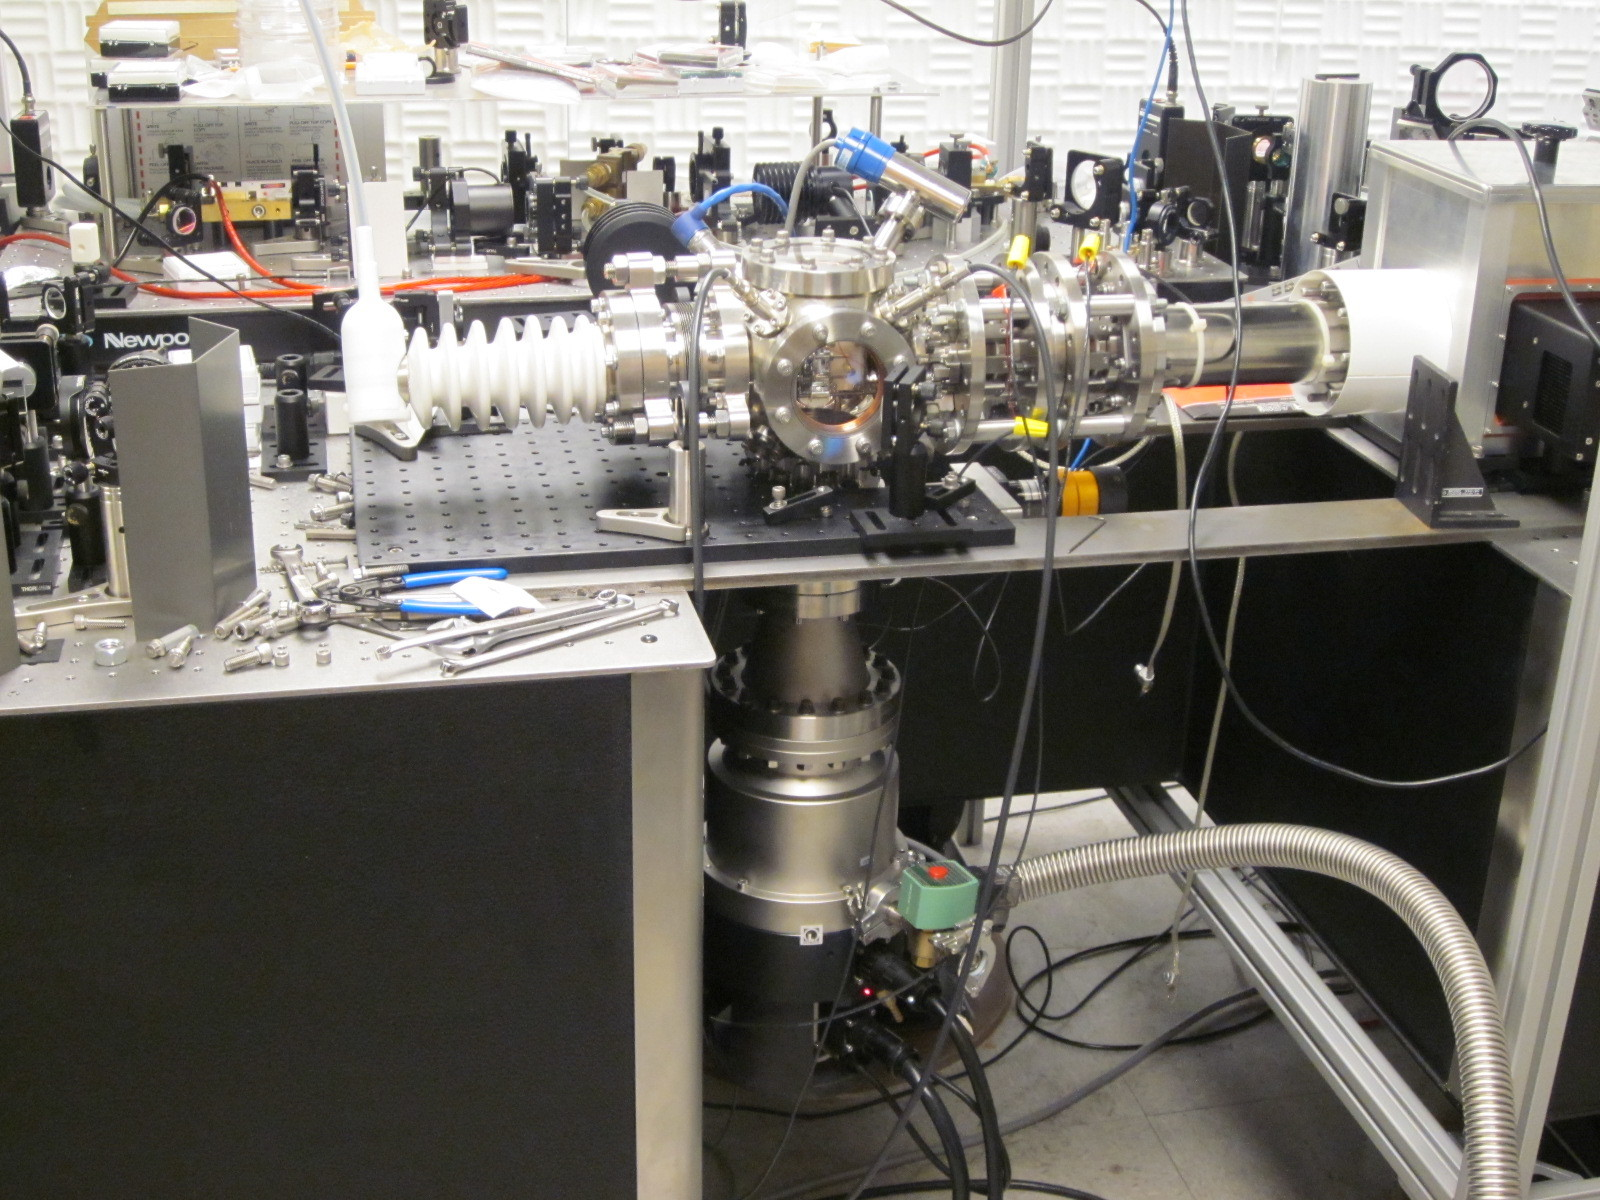
\includegraphics{inc/hardware/column.jpg}
  \caption[Picture of the prototype UEM column at UIC]{
    Picture of the majority of the prototype UEM column at UIC.
    The main vacuum chamber is laid sideways, with the high voltage (gun) at the left and the imaging system on the right.
    The magnetic levitated turbo pump hangs below the column, a scroll pump used for backing is not pictured.
    The laser system is in the background.
    All of the above is mounted on a custom shaped active vibration-canceling optical table.
    The electronic control systems are not pictured.
  }
  \label{fig:column-pic}
\end{figure}


